%! Author = mariuszindel
%! Date = 02.11.20

\section{Generics}

\subsection{Überblick}
\begin{itemize}
    \item Ohne Festlegung auf einen fixen Typen
    \begin{itemize}
        \item Erlaubt die Implementation von Strukturen ohne Verwendung von «Object»
        \item Anstelle von «Object» wird «T» verwendet
    \end{itemize}
    \item Vorteile
    \begin{itemize}
        \item Hohe Wiederverwendbarkeit
        \item Typsicherheit
        \item Performance
    \end{itemize}
    \item Boxing / Typumwandlungen fallen weg
    \item  kann generisch sein:
    \begin{itemize}
        \item Klasse / Struct / Interface / Delegates / Events
        \item Methoden
    \end{itemize}
\end{itemize}

\subsubsection{Laufzeiteffizienz}
\begin{center}
    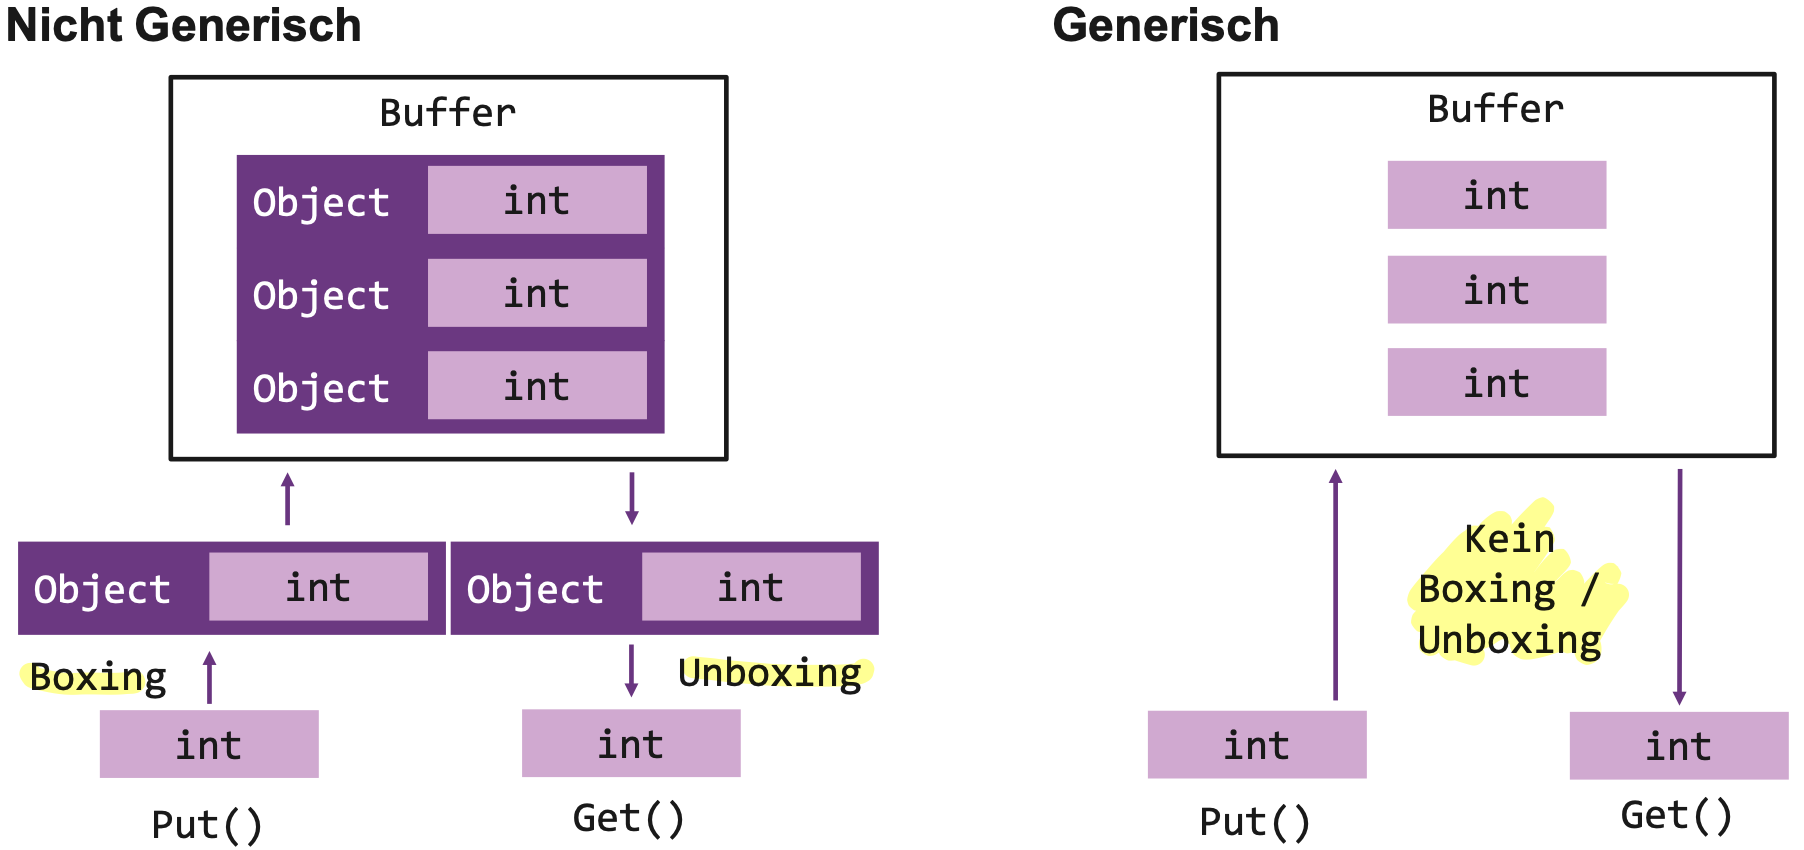
\includegraphics[scale=.25]{graphic/generics/Laufzeiteffizienz.png}
\end{center}
\vspace{-8pt}


\subsection{Type Constraints}
\begin{itemize}
    \item Mit Type Constraint «where TPriority : IComparable»
    \begin{itemize}
        \item Alle Members von «Object»
        \item Alle Members von «IComparable»
    \end{itemize}
\end{itemize}
\begin{lstlisting}
class OrderedBuffer<TElement, TPriority>
    where TPriority : IComparable
{ ... }
\end{lstlisting}

\vspace{-8pt}
\begin{center}
    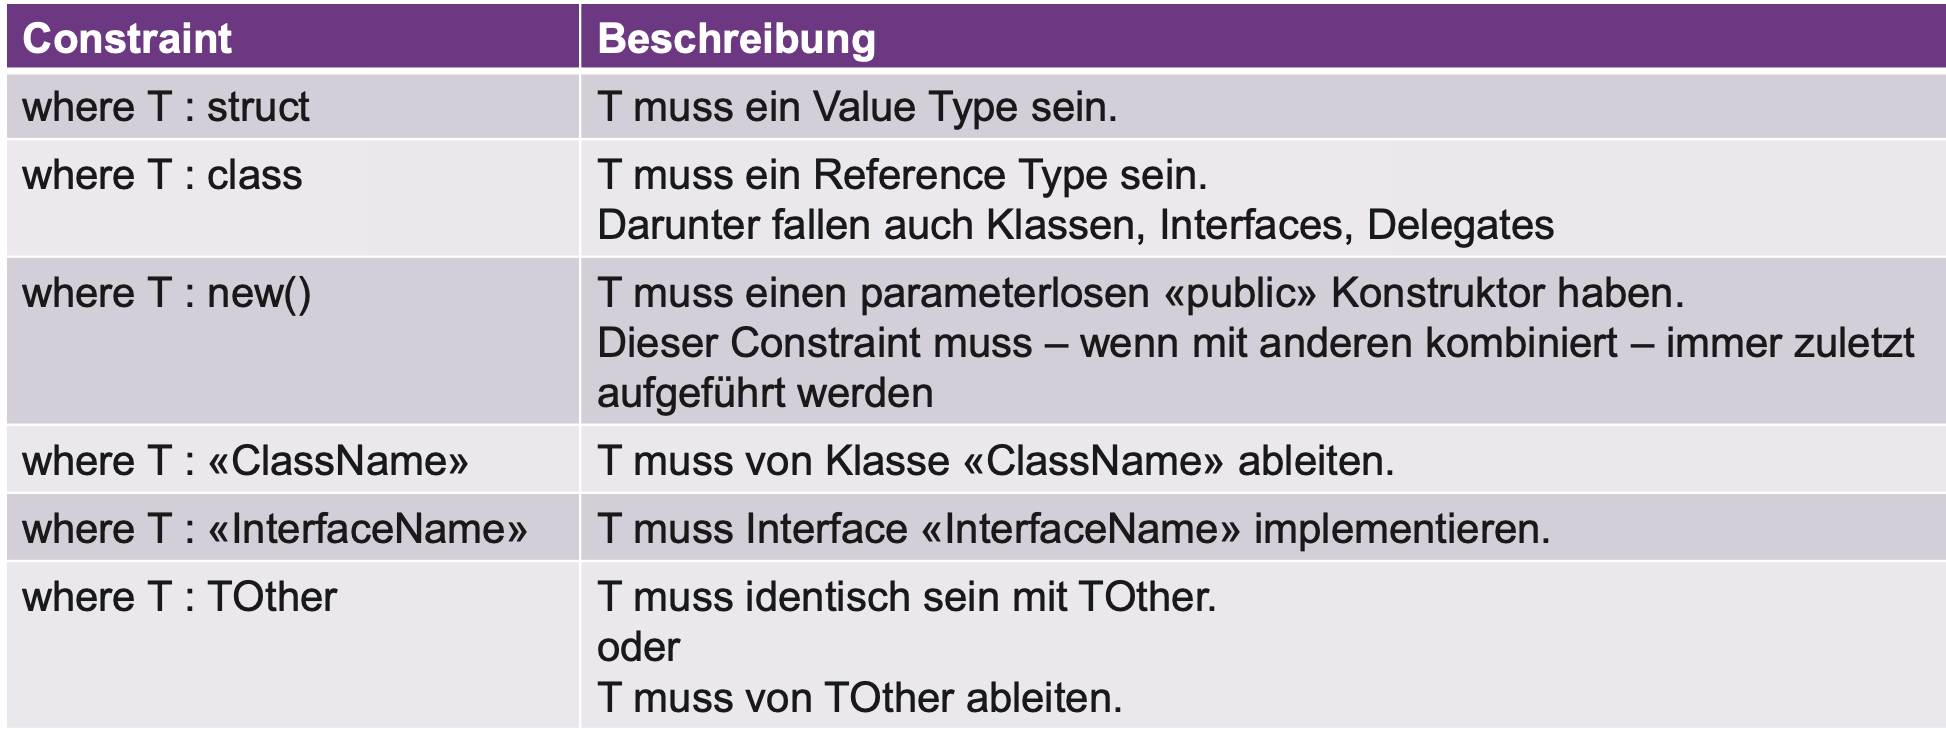
\includegraphics[scale=.23]{graphic/generics/Type Constraints.png}
\end{center}
\vspace{-8pt}

\subsubsection{T : struct}
\begin{itemize}
    \item T muss ein Value Type sein
    \item Implikationen
    \begin{itemize}
        \item T liegt auf dem Stack oder inline in einem Objekt
        \item T ist nie «null»
    \end{itemize}
\end{itemize}
\begin{lstlisting}
public void Work<T>(T source)
where T : struct
{ ... }
\end{lstlisting}

\subsubsection{T : class}
\begin{itemize}
    \item T muss ein Reference Type sein
    \item Implikationen
    \begin{itemize}
        \item T liegt auf dem Heap
        \item T kann «null» sein
    \end{itemize}
\end{itemize}
\begin{lstlisting}
public void Work<T>(T source)
where T : class
{ ... }
\end{lstlisting}

\subsubsection{T : new()}
\begin{itemize}
    \item T muss einen parameterlosen «public» Konstruktor haben
    \item Implikationen
    \begin{itemize}
        \item  T kann instanziert werden
    \end{itemize}
\end{itemize}
\begin{lstlisting}
public T GetInstance<T>()
    where T : new() {
    return new T();
}
\end{lstlisting}

\subsubsection{T : ClassName}
\begin{itemize}
    \item T muss von Klasse «ClassName» ableiten
    \item Implikationen
    \begin{itemize}
        \item T bietet alle Members von «ClassName»
    \end{itemize}
\end{itemize}
\begin{lstlisting}
public void Work<T>(T source)
where T : List<int>
{ ... }
\end{lstlisting}

\subsubsection{T : InterfaceName}
\begin{itemize}
    \item T muss Interface «InterfaceName» implementieren
    \item Implikationen
    \begin{itemize}
        \item T bietet alle Members von «InterfaceName»
    \end{itemize}
\end{itemize}
\begin{lstlisting}
public void FillList<T>(T source)
    where T : IList<int>, IEnumerable<int>
{ ... }
\end{lstlisting}

\subsubsection{T : TBase}
\begin{itemize}
    \item T muss identisch sein mit TBase oder T muss von TBase ableiten
\end{itemize}
\begin{lstlisting}

\end{lstlisting}
public void Work<T, TBase>(T a, TBase b)
where T : TBase {
    T t1 = a;
    T t2 = b; // Compilerfehler
    TBase to1 = a;
    TBase to2 = b;
}


\subsection{Vererbung}

Generische Klassen können von anderen generischen Klassen erben

\begin{itemize}
    \item Normale Klassen\\
    class MyList<T> : List { }
    \item Weitergabe des Typparameters an generische Basisklasse\\
    class MyList<T> : List<T> { }
    \item Konkretisierte generische Basisklasse\\
    class MyIntList : List<int> {}
    \item Mischform \\
    class MyIntKeyDict<T> : Dictionary<int, T> { }
    \item Typparameter werden nicht vererbt
    class MyList : List<T> { } // Compilerfehler
\end{itemize}


\subsection{Nullable Types}

\begin{itemize}
    \item «default(T)»
    \begin{itemize}
        \item Reference Types: null
        \item Value Types: 0, false oder \textbackslash0
    \end{itemize}
\end{itemize}

\begin{lstlisting}
public void NullExamples<T>() {
// Nullwerte zuweisen 
    T x1 = null;       // Compilerfehler
    T x2 = 0;          // Compilerfehler 
    T x3 = default(T); // OK
    T x4 = default;    // OK (C# 7.1)
}
\end{lstlisting}

\subsubsection{Struct «Nullable»}
\begin{center}
    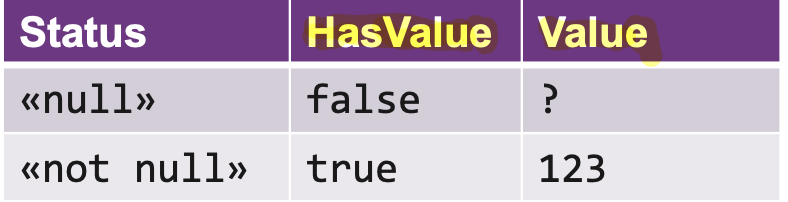
\includegraphics[scale=.3]{graphic/generics/Struct Nullable.png}
\end{center}
\begin{lstlisting}
public struct Nullable<T> where T : struct
{
    public Nullable(T value);

    public bool HasValue { get; }
    public T Value { get; }
}
\end{lstlisting}

\subsubsection{T? Syntax}
\begin{lstlisting}
int? x = null; 
double? y = null;
\end{lstlisting}


\subsubsection{Sicheres lesen \& Type Cast}
\begin{lstlisting}
// Klassisch
int x1 = x.HasValue ? x.Value: default;

// Via Methode
int x2 = x.GetValueOrDefault();

// Via Methode inkl. eigenem Default
int x3 = x.GetValueOrDefault(-1);

// Definition
private int? GetNullableInt() {
return null;
}
\end{lstlisting}


\subsubsection{?? Und ??= Operator \& Casts}

\begin{lstlisting}
// wenn i null -> -1
int i = GetNullableInt() ?? -1;

int? i = null;
i ??= 1234; // i = i ?? 1234;

\end{lstlisting}


\subsection{Generische Collections}
\begin{center}
    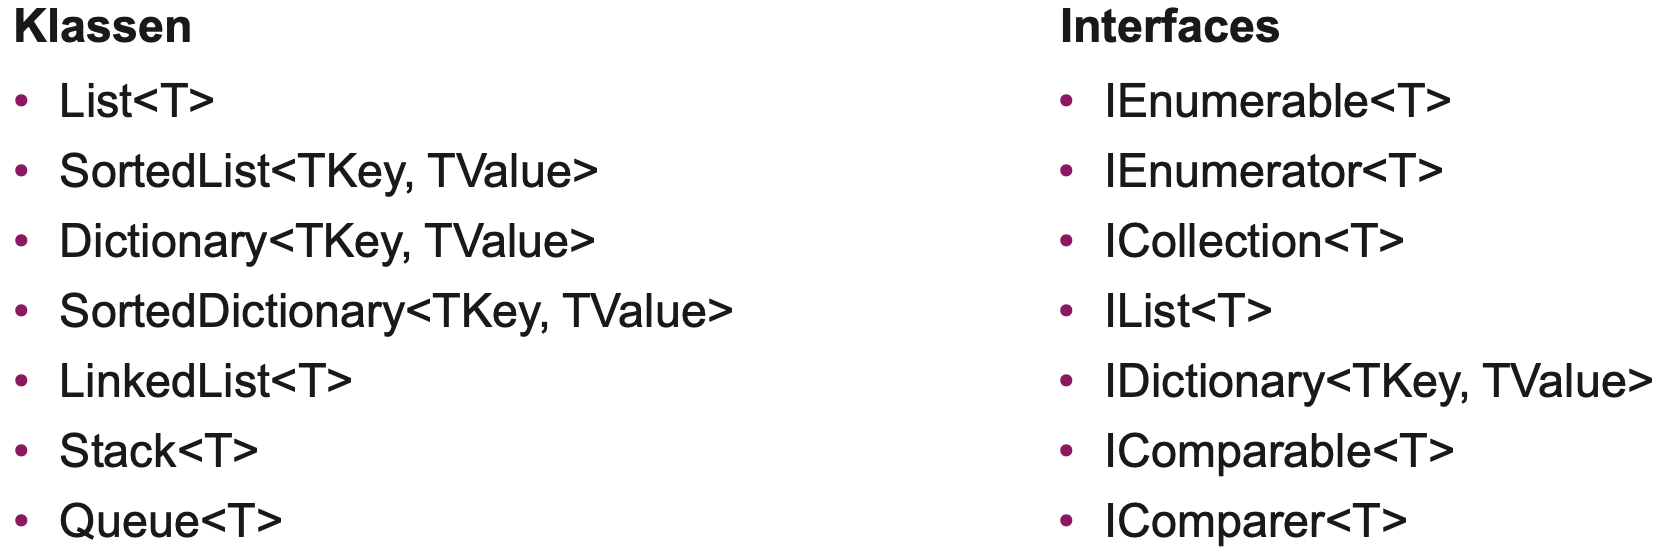
\includegraphics[scale=.24]{graphic/generics/Generische Listentypen.png}
    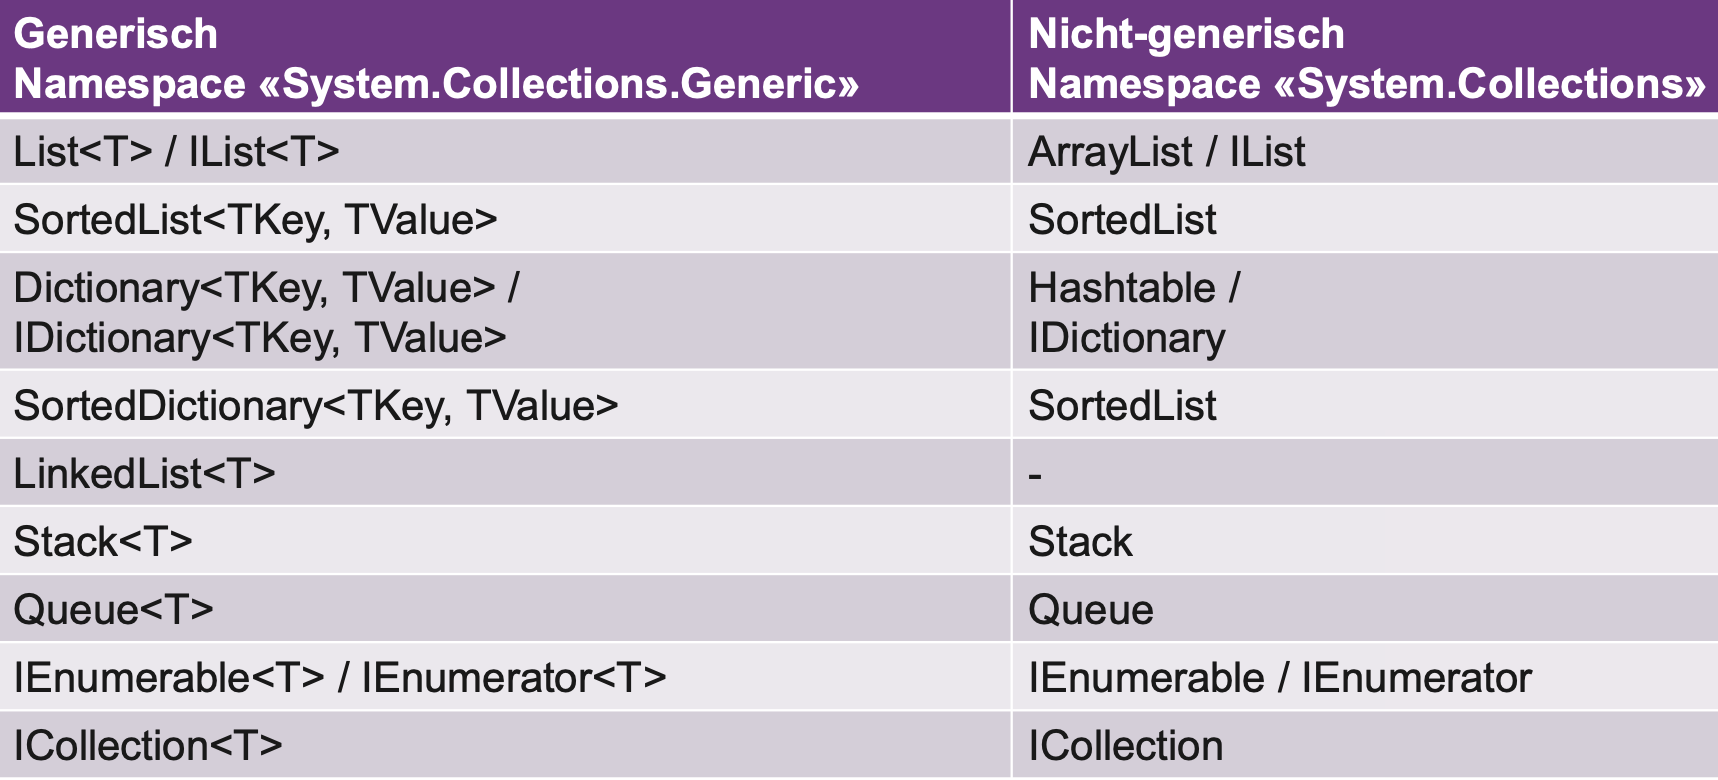
\includegraphics[scale=.24]{graphic/generics/Nicht-generische Pendants.png}
\end{center}

\newpage